The vast majority of current LLMs are based on the Transformer architecture \cite{vaswani2017attention}, which comprises a sequence of blocks traversed in a feedforward manner to predict the next token. As the capability of these models increased, attention turned to eliciting \textit{reasoning} capabilities in LLMs by increasing test-time computation, commonly through chain-of-thought (CoT) prompting \cite{wei2022chain} or reinforcement-learning-based fine-tuning, first popularized in the DeepSeek-R1 architecture \cite{guo2025deepseek}. More recently, research has explored building reasoning capabilities directly into the model architecture via \textit{recurrent looping} \cite{geiping2025scaling, wang2025hierarchical, jolicoeur2025less}, where additional test-time compute is spent by taking more recurrent steps, echoing early designs in this direction \cite{graves2016adaptive}. Despite growing empirical success, the mechanisms underlying these models remain poorly understood, as well as their benefits and limitations when compared to feedforward computation.


\begin{figure}[!t]
    \centering
    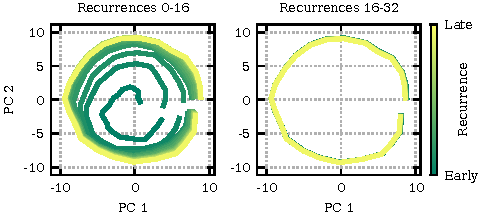
\includegraphics[width=\linewidth]{figures/splash_trajectory.pdf}
    \vspace{-0.91cm}
    \caption{\textbf{Latent states after each block in a recurrent model frequently tend towards \emph{separate} fixed points}, meaning that the application of a recurrent block tends towards a consistent trajectory in latent space.}
    \vspace{-0.5cm}
    \label{fig:random_trajectory}
\end{figure}

In this paper, we compare how feedforward and looped LLMs organize computation across (effective) depth through the lens of \textit{stages of inference} \citep{lad2024remarkable, queipo2025attention}, a perspective suggesting that LLM inference can be decomposed into several distinct computational stages. Building on prior observations that repeated application of a shared recurrent block can approach a fixed point or steady state \citep{yang2023looped, geiping2025scaling}, we show that such behavior necessarily implies one of two possibilities: either the contribution of the component Transformer blocks vanishes asymptotically, or their sequential application traces out a \textit{constant cyclic trajectory} in latent space. We further demonstrate empirically that the latter behavior arises in practice when certain architectural conditions are met, and that this appears to be emergent behavior from the Transformer architecture itself, appearing in both trained recurrent models and untrained, randomly initialized models.

\begin{tcolorbox}[colback=orange!10,
leftrule=0.5mm,top=1mm,bottom=1mm,boxrule=0.6pt]
\paragraph{Our analysis yields two key insights:}
\begin{enumerate}
    \item \Cref{sec:cyclic_similarity} establishes that many looped language models tend toward \emph{cyclic fixed-point} behavior, providing theoretical and empirical proof that this implies convergence to fixed attention patterns. \Cref{subsec:norm_and_ii} explores how specific architectural choices influence this behavior.
    \item \Cref{sec:stages_of_inference} demonstrates that these stable attention patterns mirror the ``mixing'' stages of inference learned in feedforward models. We then provide evidence in \Cref{sec:self_organising_soi} that models naturally self-organize into these stages during training, and show in \Cref{sec:stability} that stable fixed-point models successfully maintain these inference stages, whereas unstable models deviate.
\end{enumerate}
\end{tcolorbox}


